\chapter{Análisis y diseño de operadores evolutivos en esquemas de diversidad} % Main chapter title

\label{Chapter5}

\section{Introducción}
En las últimas décadas, la implementación de estrategias estocásticas para resolver problemas de optimización complejos ha ganado una gran popularidad (\cite{talbi2009metaheuristics}).
%
%Debido a esto se han propuesto diversos tipos de metaheurísticas, destacando entre las más implementadas los Algoritmos Genéticos (Genetic Algortihm - GA), Evolución Diferencial (Differential Evolution - DE), Estrategias Evolutivas (Evolution Strategies - ES), y Optimización por Enjambre de Partículas (Particle Swarm Optimization - PSO).
%
Debido a esto se han propuesto diversos tipos de metaheurísticas poblacionales, principalmente los algoritmos evolutivos (EAs) se considera una clasificación de ellas (\cite{de2006evolutionary}).
%
Existen varias categorías de los EAs, tales como algoritmos genéticos ( \cite{goldberg1989genetic}), estrategias evolutivas (\cite{beyer2002evolution}), programación genética (\cite{koza1992genetic}), programación evolutiva (\cite{dong2007evolutionary}), y otros algoritmos inspirados en la naturaleza.
%
Entre los distintos tipos de EAs, los algoritmos genéticos (GAs) son de los más populares en optimización estocástica.
%
En los estudios iniciales de GAs, las soluciones candidatas son codificadas por medio de valores binarios para simular los cromosomas \cite{molinahttp}.
%
Sin embargo en problemas de optimización con espacios de búsqueda continuos el enfoque de codificación real es mas ideal, y por lo tanto los cromosomas de los GAs son expresados por vectores de números reales.
%

Debido a su comportamiento prometedor, los EAs han sido ampliados en múltiples formas, una de ellas es el ámbito multi-objetivo siendo el tema principal de este trabajo.
%

En general, existen tres operadores evolutivos fundamentales en el ambito multi-objetivo. 
%
Estos son la selección, cruza y mutación respectivamente.
%
El operador de selección usualmente incluye dos aspectos: la selección de emparejamiento y selección del entorno (\textit{Environment Selection} - \cite{zitzler2001spea2}).
%
Inicialmente, en la \textit{selección de emparejamiento} se busca seleccionar a los individuos más prometedores, los cuales son involucrados con los operadores de variación como son los operadores de cruza y mutación.
%
Por otra parte los operadores de cruce intercambian la información de los individuos padres, con el propósito de compartir su información genética.
%
Despues de eso, el operador de mutación altera aleatoriamente la información de un individuo de forma individual, para realizar una búsqueda local, intentando encontrar individuos más aptos.
%
Por último la selección del entorno también conocido como la \textit{fase de remplazo} determina la población que sobrevive para la siguiente generación, que usualmente es seleccionada de la unión de los individuos padres y sus respectivos hijos.


Los operadores evolutivos afectan directamente el desempeño de un algoritmo evolutivo ya que dirigen el proceso de búsqueda.
%
Principalmente tienen un efecto en la diversidad de la población y por lo tanto en la calidad de las soluciones.
%
La mayoría de los operadores evolutivos están diseñados para esquemas de corto plazo, ignorando la necesidad de promover y preservar la diversidad de la población en esquemas de largo plazo.
%

Específicamente, se considera al operador de cruce un punto clave del algoritmo evolutivo (\cite{Joel:OperatorAHX}), ya que está diseñado para intensificar o explorar en base a la posición de los individuos padre.
%
Además algunos operadores son considerados más agresivos o disruptivos que otros, y usualmente algunos requieren parámetros de usuario.

%
Particularmente, en este capítulo se desea analizar el comportamiento del operador de Cruce Binario Simulado (SBX) y del operador de evolución diferencial (DE) en el ámbito multi-objetivo junto con esquemas donde se administra la diversidad de forma explícita.
%

%
Inicialmente se revisa la taxonomía de los operadores de cruce, principalmente es analizado el operador SBX en esquemas a largo plazo, posteriormente se propone una modificación para promover la diversidad por parte de las soluciones.
%
Adicionalmente, se hace un análisis de los operadores de evolución diferencial y se muestran las dificultades que existen al considerar mecanismos donde la diversidad es mantenida de forma explícita.
%
Finalmente se realiza una propuesta de evolución diferencial para las propuestas algorítmicas de este documento.

\section{Operadores de cruce}

Usualmente, los operadores de cruce tienden a promover mayor diversidad cuando se consideran padres distantes, de forma contraria cuando los padres están suficientemente cercanos existe un efecto de intensificación.
%
De esta forma, los operadores de cruce son métodos adaptativos que dependen en la diversidad mantenida dentro de la población.
%
En el caso de la codificación real, se han propuesto varios operadores de cruce (\cite{herrera2003taxonomy}), que pueden ser clasificados como centrados en los padres o en la media, en base a la región donde existe la tendencia de crear a los individuos hijo.
%
El operador de Cruce Binario Simulado (Simulated Binary Crossover - SBX  \cite{deb1999self}) es probablemente uno de los más utilizados.
%
En la versión inicial del SBX, se definió la forma de intercambiar la información para una variable.
%
Tomando en cuenta las características de las distribuciones involucradas, el operador SBX se clasifica como un operador de cruce centrado en los padres.
%
Por lo tanto, este tiende a crear soluciones cercanas a los padres.
%
Sin embargo, la forma de extender al operador SBX a problemas de varias variables no se ha discutido en detalle.
%
Como resultado, se han propuesto diferentes implementaciones para hacer frente a problemas de que consideran muchas variables.
%


Los operadores de cruce están diseñados con el objetivo de generar soluciones candidatas utilizando la información de dos o más soluciones padres.
%
Dado que existen múltiples operadores, se han propuesto varias taxonomías para clasificarlos \textit{Centrados en los Padres} y los \textit{Centrados en la media} (\cite{jain2011parent}).
%
En los operadores centrados en los padres, las soluciones hijas son creadas alrededor de cada solución padre, mientras que en los operadores centrados en la media, las soluciones hijas son creadas alrededor de la media de las soluciones padres.
%

Adicionalmente, otra taxonomía clasifica a los operadores en \textit{Orientados en las variables} y \textit{Orientados en los vectores}.
%
En la categoría de los operadores orientados en las variables, cada variable de las soluciones padre es combinada de forma independiente mediante una probabilidad para crear nuevos valores.
%
Algunos de los operadores que pertenecen a esta categoría son \textit{blend crossover} (BLX - \cite{eshelman1993real} ), y SBX.
%
Los operadores orientados en los vectores, son diseñados para considerar la dependencia entre las variables.
%
Normalmente, aplican una combinación lineal de todas las variables.
%
Algúnos de los operadores que pertencen a esta categoría son \textit{unimodal normally distribuited crossover} (UNDX - \cite{Joel:UNDX}) y el \textit{simplex crossover} (SPX - \cite{Joel:DE_Storn_SPX} ).
%


\subsection{Cruce Binario Simulado (SBX)}

Es uno de los operadores de cruce más utilizados en los MOEAs y es clasificado como centrado en los padres, particularmente tiene la propiedad de crear cualquier valor en el espacio de búsqueda combinando dos individuos padres.
%
Así de dos individuos padres ($p_1$, $p_2$) se generan dos hijos ($c_1$, $c_2$) en base a una distribución de probabilidad.
%
Entonces para tener un control al incluir este operador en el algoritmo se define la probabilidad por medio del factor de dispersión $\beta = | c_1 - c_2| / |p_1 - p_2|$.
%
El parámetro para que el usuario pueda controlar la forma de la distribución de probabilidad es el índice de distribución $\eta_c$, éste determina la apertura de la distribución, y por tanto, la capacidad de exploración.
%
Específicamente, un índice de distribución pequeño induce una mayor probabilidad de construir soluciones hijas alejadas de los padres, mientras que con un índice de distribución elevado, la probabilidad de crear soluciones hijas más similares a los padres se incrementa. 
%
%
El efecto de $\eta_c$ es ilustrado en la Figura \ref{fig:Density_SBX}, donde se muestran las funciones de densidad de dos índices de distribución distintos.
%
Específicamente los círculos representan a los padres, y se puede apreciar que con $\eta_c=5$, la probabilidad de crear soluciones más cercanas a los padres es mayor que con $\eta_c=2$.
\begin{figure*}[!t]%[H]
\centering
\begin{tabular}{cc}
   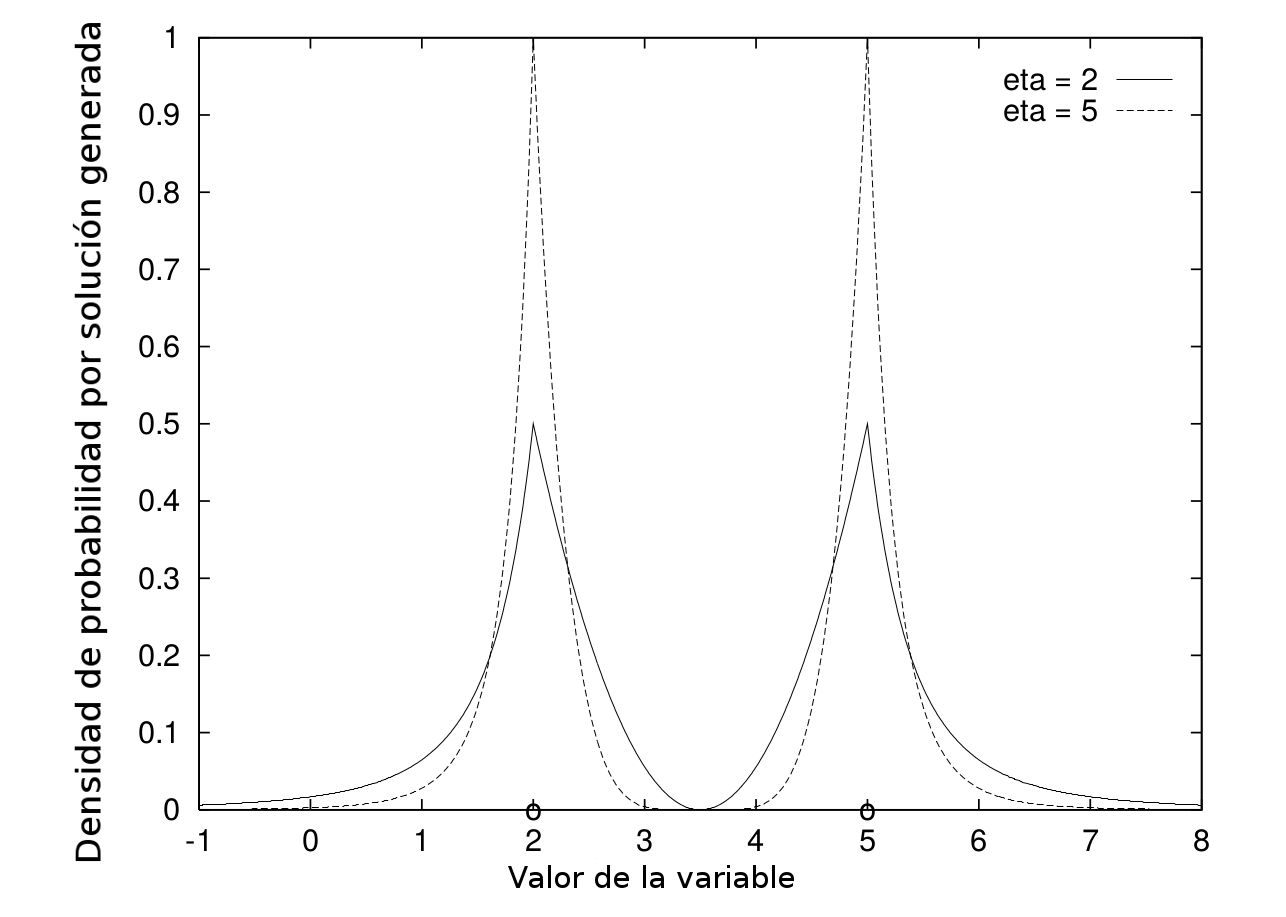
\includegraphics[width=0.5\textwidth]{Figures_Chapter6/DensitySBX.png} &
\end{tabular}
\caption{Función de densidad del operador SBX con índices de distribución 2 y 5.}
\label{fig:Density_SBX}
%\caption{Probability density function SBX with indexes of distribution 1,2 and 5. The red point is a Parent solution.}
\end{figure*}


%
%(\cite{herrera2003taxonomy})
Entonces, la probabilidad de distribución genérica para crear el valor de un individuo hijo es definido en función del parámetro de dispersión $\beta \in [0, \infty]$ de la forma:
\begin{equation}
    P(\beta)= 
\begin{cases}
     0.5(\eta_c + 1)\beta^{\eta_c},& \text{si} \quad \beta \leq 1\\
     0.5(\eta_c + 1) \frac{1}{\beta^{\eta_c + 2}} ,& \text{de otra forma}
\end{cases}
\end{equation}
Además de la propiedad para preservar una relación entre la media de los valores padres e hijos ($c_1 + c_2 = p_1 + p_2$), la distribución de probabilidad ofrece las siguiente propiedades:
\begin{itemize}
\item Los valores de las soluciones hijas son equidistantes de los padres.
\item Existe una probabilidad no nula de generar una solución hija en cualquier parte en el espacio independientemente de donde se localicen los padres.
\item La probabilidad de crear un par de soluciones hijas dentro del rango de las soluciones padres es idéntica a la probabilidad de crear dos soluciones hijas fuera de dicho rango.
\end{itemize}

Para dos valores de los individuos padres ($p_1$, $p_2$), pueden ser creados dos valores  de los hijos ($c_1$, $c_2$) como combinación lineal de los valores padres con un número aleatorio $u \in [0, 1]$ de la forma (\cite{Joel:SBX1994}):
\begin{equation} \label{eq:generar_ind}
\begin{split}
c_1 &= 0.5(1 + \beta(u))p_1 + 0.5(1 - \beta(u)) p_2 \\
c_2 &= 0.5(1 - \beta(u))p_1 + 0.5(1 + \beta(u)) p_2
\end{split}
\end{equation}
%
Así, para realiza la simulación del parámetro $\beta(u)$, primero es generado un número aleatorio $u \in [0, 1]$, y se utiliza en la siguiente fórmula:
\begin{equation} \label{eq:Parametro_beta}
    \beta(u)= 
\begin{cases}
     (2u)^{\frac{1}{\eta_c+1}},& \text{si} \quad u \leq 0.5,\\
     	(\frac{1}{2(1-u)})^{\frac{1}{\eta+1}} ,& \text{de otra forma}
\end{cases}
\end{equation}

Se puede observar que la forma de la distribución no es afectada por los límites de cada variable, en base a este inconveniente, los autores \cite{deb1999self} modificaron la ecuación (\ref{eq:Parametro_beta}) de forma que exista una probabilidad cero de crear individuos afuera del rango específico, por lo tanto se puede calcular $\beta(u, a)$ en función de un número aleatorio $u \in [0,1]$ de la forma:
\begin{equation} \label{eq:sbx_bounds}
    \beta(u, a)= 
\begin{cases}
     (2u(1-\rho_a))^{\frac{1}{\eta_c+1}},& \text{si} \quad u \leq 0.5/(1-\rho_a),\\
     	(\frac{1}{2(1-u(1-\rho_a))})^{\frac{1}{\eta+1}} ,& \text{de otra forma}
\end{cases}
\end{equation}

donde $a=x_i^{(L)}$ es el límite inferior y $b=x_i^{(U)}$ es el límite superior, y $\rho_a = 1/(2 \beta_a^{\eta_c+1})$, donde $\beta_a = 1 +(p_1 - a)/(p_2 - p_1)$.
%
Similarmente, $\rho_b$ es calculado reemplazando $\beta_a$ por $\beta_b =  1 + (b - p_2)/(p_2 - p_1)$, así $\beta(u, b)$ es calculado con la ecuación (\ref{eq:sbx_bounds}), generando así dos individuos hijo en base a sus respectivas funciones de distribución $\beta(u,a)$ y $\beta(u,b)$.
%
En la práctica, se debe evitar que todas las variables sean cambiadas de forma simultánea, por lo que en las implementaciones actuales cada variable se cambia con una probabilidad igual a 0.5, mientras que en el resto de casos los valores se heredaran sin ser alterados (\cite{Joel:NSGAII,Joel:jMetal}).
%
Además, por la forma en que se heredan las variables, normalmente se aplican intercambios entre las variables de los hijos, que resultan en reflexiones y son analizados posteriormente.
%
Por último, cabe destacar que no existen versiones del operador SBX en las que en lugar de usar dicha probabilidad fija en 0.5, esta sea cambiada a lo largo de la ejecución.

 \begin{algorithm}[H]
\algsetup{linenosize=\tiny}
\scriptsize
\caption{Operador de Cruce Binario Simulado (SBX)}
\label{alg:SBX_Operator}
\begin{algorithmic}[1]
    \STATE Entrada: Individuos Padre ($P_1, P_2$), Indice de distribución ($\eta_c$), Probabilidad de cruza ($P_c$).
    \STATE Salida: Individuos hijo($C_1, C_2$).
    \STATE $r_1 \leftarrow U[0, 1]$.
    \IF{ $r_1 \leq P_c$}
       \FOR{ cada variable d}
	\IF{ $U[0, 1] \leq 0.5$}
		 \STATE $a = LowBound(d)$.	
		 \STATE $b = UpperBound(d)$.    
		 \STATE $ r_2 \leftarrow U[0, 1]$.
		 \STATE $\beta_a = 1 +(p_1 - a)/(p_2 - p_1)$.
		 \STATE $\rho_a = 1/(2 \beta_a^{\eta_c+1})$.
		 \STATE Utilizar $r_2$ y $\rho_a$ en la ecuación \ref{eq:sbx_bounds} para generar $\beta(u,a)$.  
		 \STATE Generar a $C_1(d)$ utilizando $\beta(u, a)$ en la ecuación \ref{eq:generar_ind}. 
		 \STATE $\beta_b = 1 +(b - p_2)/(p_2 - p_1)$.
		 \STATE $\rho_b = 1/(2 \beta_b^{\eta_c+1})$.
		 \STATE Utilizar $r_2$ y $\rho_b$ en la ecuación \ref{eq:sbx_bounds} para generar $\beta(u,b)$. 
		 \STATE Generar a $C_2(d)$ utilizando $\beta(u, b)$ en la ecuación \ref{eq:generar_ind}.
		 \IF{$ U[0, 1]  \leq 0.5$} \tikzmark{top}
			 \STATE Intercambiar los valores de $C_1(d)$ con $C_2(d)$. \tikzmark{right}
		 \ENDIF \tikzmark{bottom}
        \ELSE \tikzmark{top2}
	   \STATE $C_1(d) = P_1(d)$. \tikzmark{right2}
	   \STATE $C_2(d) = P_2(d)$.
        \ENDIF \tikzmark{bottom2}
       \ENDFOR
    \ELSE
	\STATE $C_1 = P_1$
	\STATE $C_2 = P_2$
    \ENDIF
\end{algorithmic}
\AddNote{top}{bottom}{right}{En esta sección se implementa la reflexión.}
\AddNote{top2}{bottom2}{right2}{En esta sección es controlada la similitud.}
\end{algorithm}


%
\subsection{Análisis operador de cruce SBX}

%
La implementación más utilizada del operador SBX se encuentra integrada en el NSGA-II publicada por \cite{Joel:NSGAII}.
%
Este procedimiento está indicado en el algoritmo \ref{alg:SBX_Operator}, donde destacan dos aspectos clave.
%
El primero está relacionado con la similitud entre los individuos padre y los hijo (líneas 22 y 23).
%
En dicha implementación los valores de las soluciones hijas son heredadas directamente de las soluciones padre con una probabilidad fija igual a 0.5, mientras que el resto de las variables son modificadas mediante la distribución de probabilidad propia del SBX.
%
En consecuencia la similitud que existe entre los padres y los hijos depende altamente del número de variables que se consideran en el problema de optimización, pues el incremento de la dimensionalidad involucra la creación de soluciones más distantes.

El segundo punto clave, que nunca ha sido analizado en detalle, está relacionado con el conjunto de reflexiones que se realizan (líneas 18 - 20).
%
%
Después de generar los dos valores que deben ser heredados en los dos hijos, dichos valores son intercambiados entre sí con una probabilidad fija del 0.5.
%
En consecuencia, cada vez que las variables son intercambiadas se realiza una reflexión, que puede inducir grandes distancias entre los padres y los hijos, a pesar de que el SBX es considerado como un cruce centrado en los padres.
%
La parte izquierda de  la Figura~\ref{fig:Simulations_Index_20} ilustra  este comportamiento en el operador SBX para dos y tres variables.
%
En esta figura, los padres están identificados con dos puntos rojos, y se ejecutó el operador SBX diez mil veces.
%
Cada uno de los puntos de color negro es una solución hija, con lo que esta figura ilustra las zonas en las que se tienden a generar a los hijos.
%
Se puede ver que los valores de cada variable siempre están cercanos a uno de los valores asociados a las variables de los padres. 
%
Sin embargo, debido al proceso de intercambio de valores, las soluciones hijas no siempre se encuentran cercanas a los padres.
%
Particularmente, en el caso de dos dimensiones mostrado, se crean soluciones en la esquina superior izquierda y en la esquina inferior derecha, mientras que los padres están es las esquinas opuestas.
%
A medida que aumenta el número de dimensiones $d$, la probabilidad de que siempre o nunca haya intercambios, y que por tanto, la nueva solución esté cercana a uno de los padres es $k^{d} + (1-k)^{d}$, con lo que se produce un decremento exponencial respecto al número de dimensiones.
%
%
En consecuencia, las reflexiones provocan un alto grado de exploración.
En algunos MOPs con alta dimensionalidad en el espacio de las variables, esto podría representar un inconveniente porque las reflexiones localizan soluciones hijas en cada esquina del hipercubo mínimo que contiene a las soluciones padre, lo que significa que el operador original podría inducir un nivel muy bajo de intensificación.

El inconveniente relacionado con las reflexiones puede ser manejado parcialmente implementando restricciones de emparejamiento que traten de cruzar exclusivamente a soluciones similares. 
%
Bajo esta condiciones, el hipercubo sería de menor tamaño, con lo que se induciría un mayor grado de intensificación.
%
Esta puede ser una de las razones por las que el MOEA/D, que incorpora restricciones de apareamiento, ha sido capaz de resolver muchos problemas de forma exitosa.
%
En este trabajo, se trata de resolver esta problemática eliminando el intercambio de variables, así como realizando otras modificaciones en el SBX que se describen en la siguiente sección.
%
La ventaja de esta segunda alternativa es que se puede incorporar de forma sencilla en cualquier MOEA.
%

\begin{figure*}
\centering
\begin{tabular}{cc}
   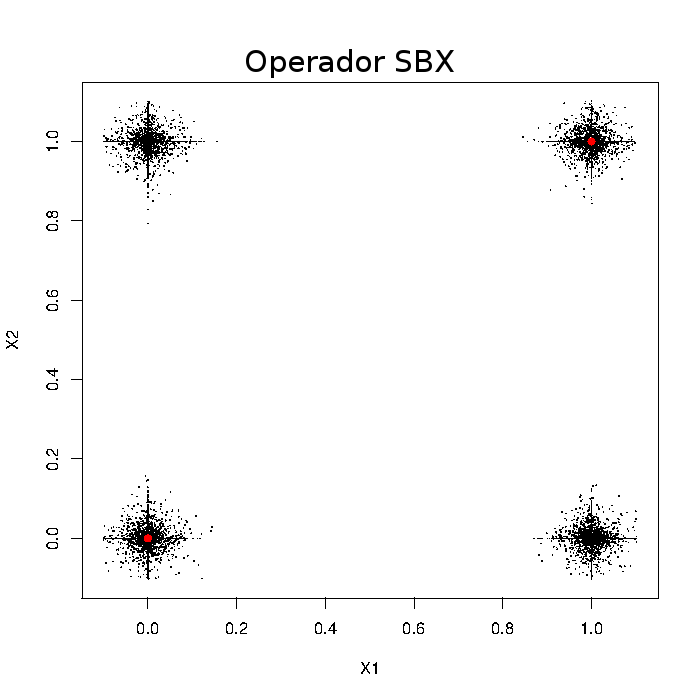
\includegraphics[width=0.3\textwidth]{Figures_Chapter6/SBX_2D_Index_20.png} &
   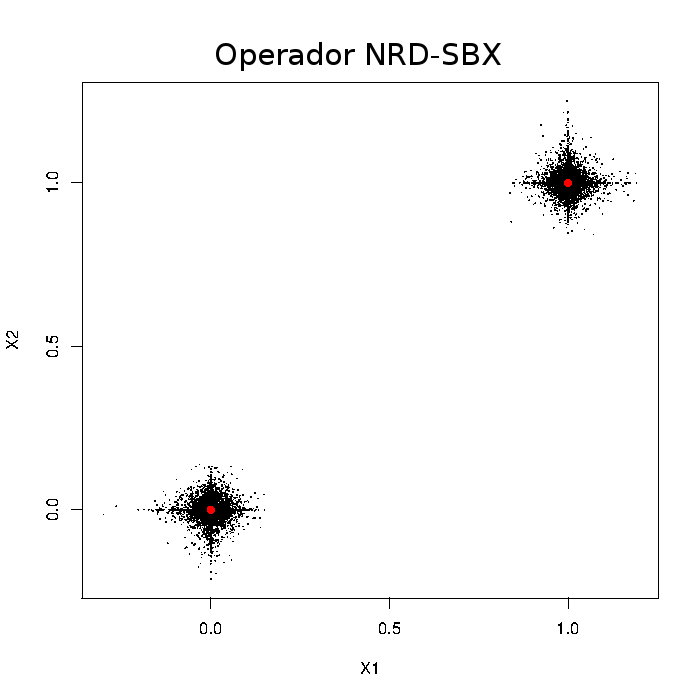
\includegraphics[width=0.3\textwidth]{Figures_Chapter6/DSBX_2D_Index_20.png} \\   
   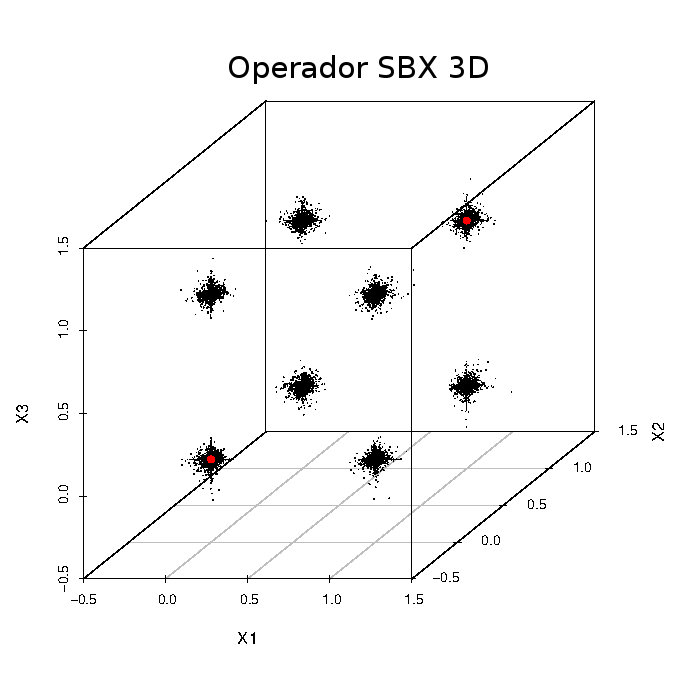
\includegraphics[width=0.3\textwidth]{Figures_Chapter6/SBX_3D_Index_20.png} &
   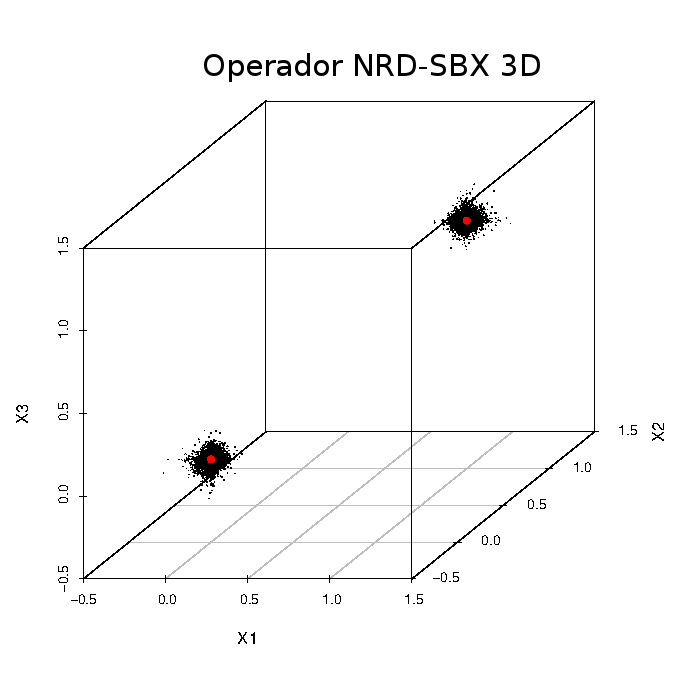
\includegraphics[width=0.3\textwidth]{Figures_Chapter6/DSBX_3D_Index_20.png}  
\end{tabular}
\caption{En la columna izquierda se presenta la simulación del operador  SBX y en la columna de la derecha se presenta el operador NRD-SBX, ambas distribuciones con un índice de distribución de 20.}
%\caption{Simulations SBX left column and NRD-SBX right column with index distribution 20}
\label{fig:Simulations_Index_20}
\end{figure*}

\subsection{Propuesta del operador SBX basado en esquemas de diversidad}
%
Tomando en cuenta el análisis previo, así como el deseo de adaptar el operador a los requerimientos de las diferentes fases de optimización, se diseñó e implementó un nuevo operador de cruce indicado en el algoritmo \ref{alg:NRDSBX_Operator}, que se denominada operador Dinámico sin Reflexiones basado en el Cruce Binario Simulado (NRD-SBX).
%
NRD-SBX realiza dos modificaciones al operador SBX descrito anteriormente.

%
En primer lugar, en el NRD-SBX, la probabilidad de intercambiar variables se fija a cero, con lo que nunca aparecen las reflexiones propias del SBX original. 
%
El efecto de este cambio se muestra en la parte derecha de la Figura \ref{fig:Simulations_Index_20}, en la que podemos ver que ahora todos los hijos quedaron localizados en regiones cercanas a los padres.
%
Esto implica un mayor grado de intensificación.
%
Es importante hacer notar la diferencia entre el operador modificado SBX y un operador de mutación.
%
La distancia entre padres e hijos en el NRD-SBX es proporcional a la distancia entre los padres, mientras que los operadores de mutación sólo consideran la información de una solución padre.

La segunda modificación del NRD-SBX está relacionada con la cantidad de variables que se heredan sin modificarse.
%
El operador SBX hereda directamente los valores que corresponden a los padres con una probabilidad igual a 0.5.
%
Esto podría limitar el grado de exploración, 
especialmente en las primeras generaciones.
%
Para evitar esta problemática, el operador NRD-SBX altera la probabilidad de heredar sin modificar las variables de los padres durante la ejecución del algoritmo.
%
Particularmente, se implementa un modelo dinámico lineal, donde en la primera generación, esta probabilidad es asignada a cero y con el transcurso de las generaciones, la probabilidad se incrementa de manera lineal, de forma que cuando ha transcurrido la mitad de las generaciones la probabilidad es igual a 0.5.
%
A partir de este momento, y hasta el final de la ejecución, se mantiene fija la probabilidad a 0.5.
%
Esta regla tiende a ir disminuyendo paulatinamente el número de variables que se heredan sin realizar modificaciones, con lo que en las primeras fases se induce un mayor grado de exploración y las últimas fases, se induce un mayor grado de intensificación.
%
La Figura \ref{fig:Simulations_TimeLine}, muestra para el caso de dos dimensiones, una simulación heredando directamente las variables con una probabilidad de 0, 0.25 y 0.50.
%
Se puede apreciar que con probabilidades bajas (fases iniciales de la optimización) se exploran más zonas, mientras que en las fases finales se tienden a crear muchas soluciones que comparten valores con los padres, siendo este un paso mucho más intensificador.
%
Cabe destacar que el comportamiento final en el que se mantienen bastantes variables sin cambiar, es deseado con MOPs en los que las variables son independientes entre sí.
%
Sin embargo, en los problemas que involucran dependencia entre las variables, utilizar modificaciones de este tipo puede llevar a que el algoritmo se quede estancado en óptimos locales de baja calidad.
%


\begin{figure*}[t]%[H]
\centering
\begin{tabular}{ccc}
   %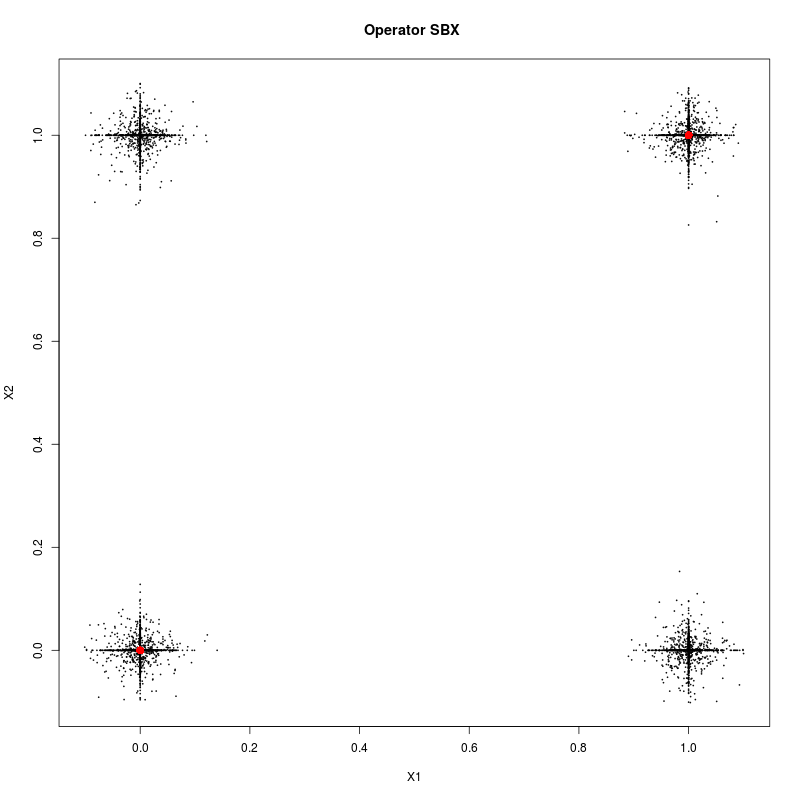
\includegraphics[width=0.3\textwidth]{Figures_Chapter6/SBX_2D_First.png} &
   %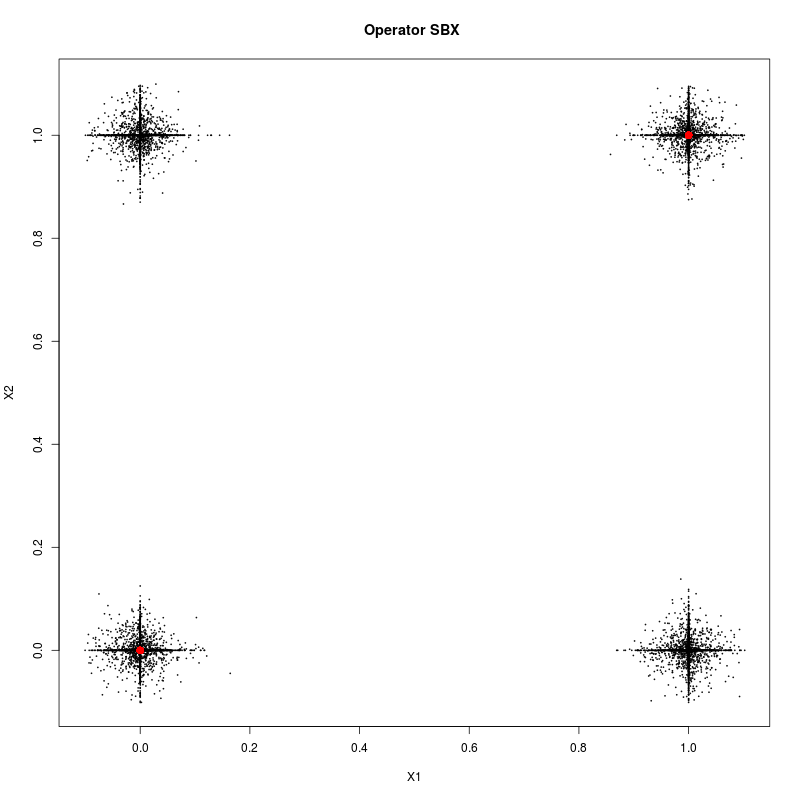
\includegraphics[width=0.3\textwidth]{Figures_Chapter6/SBX_2D_Second.png} &   
   %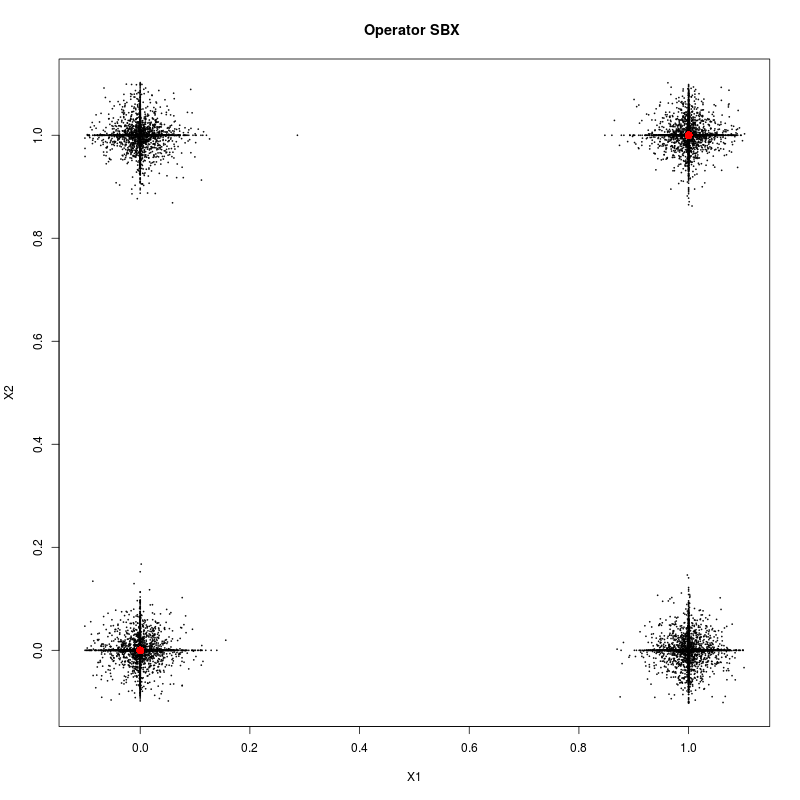
\includegraphics[width=0.3\textwidth]{Figures_Chapter6/SBX_2D_Third.png} \\
   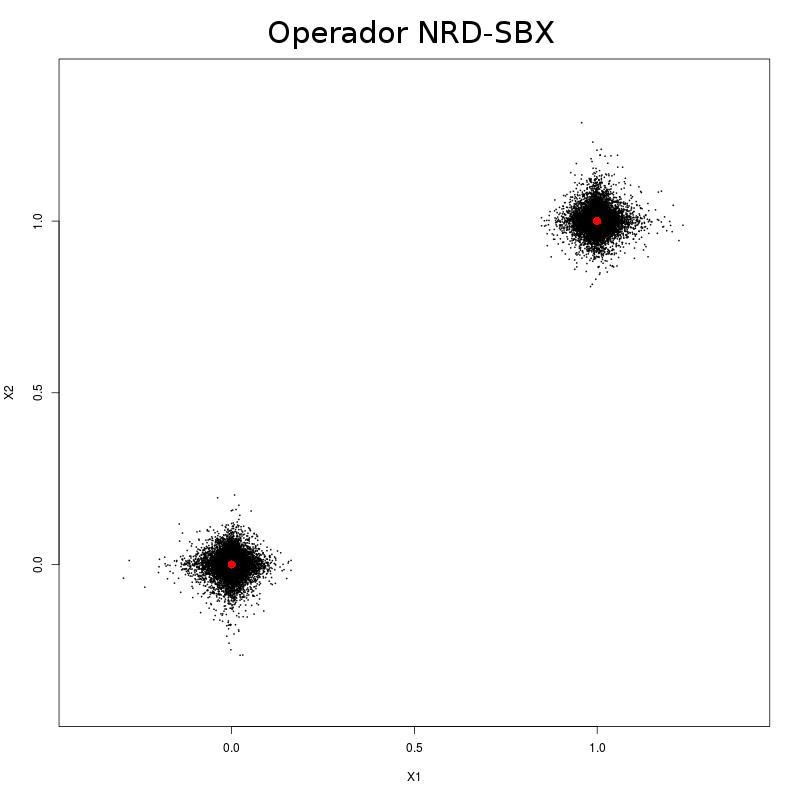
\includegraphics[width=0.3\textwidth]{Figures_Chapter6/DSBX_2D_First.png} &
   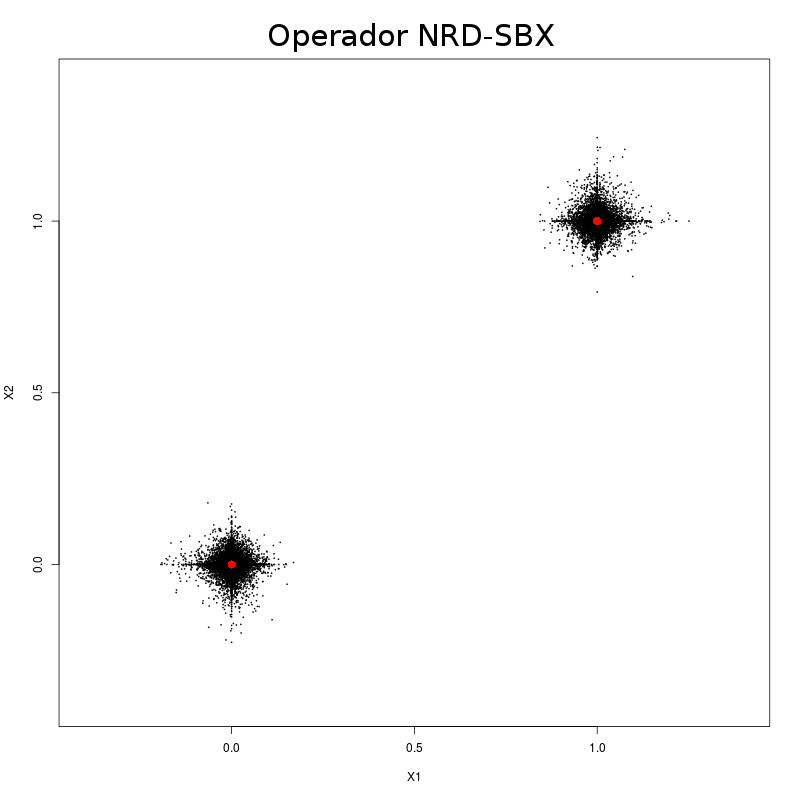
\includegraphics[width=0.3\textwidth]{Figures_Chapter6/DSBX_2D_Second.png} & 
   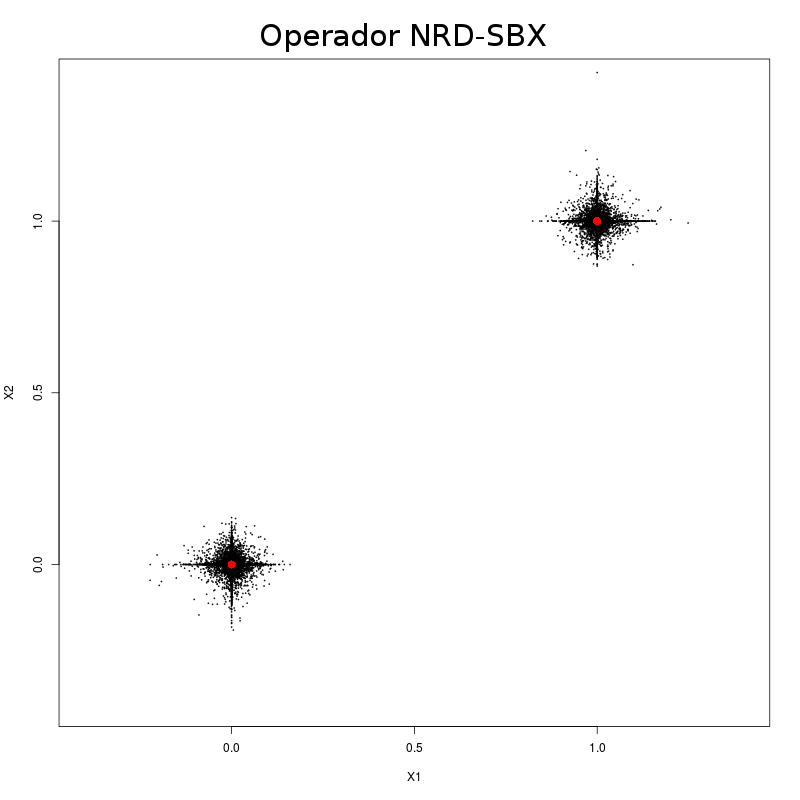
\includegraphics[width=0.3\textwidth]{Figures_Chapter6/DSBX_2D_Third.png} 
\end{tabular}
\caption{Simulación del operador SBX con la probabilidad de heredar directamente las variables con 0\%, 25\% y 50\% respectivamente. Los puntos rojos representan a los individuos padres.}
%\caption{Simulations of SBX  the variables to $0\%$, $33\%$ and $50\%$ of total of generations. The red points represent the parents solutions}
\label{fig:Simulations_TimeLine}
\end{figure*}


 \begin{algorithm}[t]
\algsetup{linenosize=\tiny}
\scriptsize
\caption{Operador Dinámico sin Reflexiones basado en el Cruce Binario Simulado (NRD-SBX)}
\label{alg:NRDSBX_Operator}
\begin{algorithmic}[1]
    \STATE Entrada: Individuos Padre ($P_1, P_2$), Indice de distribución ($\eta_c$), Probabilidad de cruza ($P_c$), Generación actual ($t_i$).
    \STATE Salida: Individuos hijo($C_1, C_2$).
    \STATE $\delta = min( \frac{1}{2} ,\frac{t_i}{Total\quad Generaciones})$
    \STATE $r_1 \leftarrow U[0, 1]$.
    \IF{ $r_1 \leq P_c$}
       \FOR{ cada variable d}
	\IF{ $U[0, 1] \geq \delta$}
		 \STATE $a = LowBound(d)$.	
		 \STATE $b = UpperBound(d)$.    
		 \STATE $ r_2 \leftarrow U[0, 1]$.
		 \STATE $\beta_a = 1 +(p_1 - a)/(p_2 - p_1)$.
		 \STATE $\rho_a = 1/(2 \beta_a^{\eta_c+1})$.
		 \STATE Utilizar $r_2$ y $\rho_a$ en la ecuación \ref{eq:sbx_bounds} para generar $\beta(u,a)$.  
		 \STATE Generar a $C_1(d)$ utilizando $\beta(u, a)$ en la ecuación \ref{eq:generar_ind}. 
		 \STATE $\beta_b = 1 +(b - p_2)/(p_2 - p_1)$.
		 \STATE $\rho_b = 1/(2 \beta_b^{\eta_c+1})$.
		 \STATE Utilizar $r_2$ y $\rho_b$ en la ecuación \ref{eq:sbx_bounds} para generar $\beta(u,b)$. 
		 \STATE Generar a $C_2(d)$ utilizando $\beta(u, b)$ en la ecuación \ref{eq:generar_ind}.
        \ELSE \tikzmark{top2}
	   \STATE $C_1(d) = P_1(d)$. \tikzmark{right2}
	   \STATE $C_2(d) = P_2(d)$.
        \ENDIF \tikzmark{bottom2}
       \ENDFOR
    \ELSE
	\STATE $C_1 = P_1$
	\STATE $C_2 = P_2$
    \ENDIF
\end{algorithmic}
\AddNote{top2}{bottom2}{right2}{La similitud se controla dinámicamente.}
\end{algorithm}


%----------------------------------------------------------------------------------------
%

\subsection{Operadores de evolución diferencial (DE)}

Evolución Diferencial (DE) es considerado como un algoritmo evolutivo, y es ampliamente utilizado en muchas aplicaciones del mundo real, debido a su simplicidad, eficiencia y competitividad.
%
Principalmente, por su efectividad ante otros algoritmos evolutivos ha sido objeto de estudio, además han surgido variantes del mismo, como son esquemas adaptativos (\cite{zhang2009jade}), definición de vecindades basadas con mutaciones, operadores híbridos (\cite{Joel:OperatorAHX}), tamaños de poblaciones dinámicas, DE paralelas, entre otros.

%
Estas variantes de DE, se desarrollaron para tratar distintos problemas en el area de optimización, como son los problemas multimodales y/o no separables (\cite{kukkonen2009performance}).
%
Particularmente, el efecto de evolución diferencial en el ámbito multi-objetivo es realmente importante y en parte está relacionado al caso multimodal.
%


Evolución diferencial utiliza la ubicación de los individuos en el espacio de búsqueda, por lo cual es importante que al inicio del proceso evolutivo los individuos estén bien distribuidos en el espacio factible.
%
De otra forma, si los individuos están muy cercanos entre sí, el proceso de búsqueda puede estancarse en algunas regiones, como resultado se podría converger prematuramente, sin la capacidad de generar individuos en otras zonas del espacio factible.
%
Además, si la población está agrupada en una región del espacio de búsqueda, no se podrán generar largos desplazamientos en el espacio factible.
%
Se han diagnosticado algunas debilidades de DE, principalmente en problemas no separables, es decir, donde existe un grado de dependencia elevado entre los parámetros.
%
Se ha observado que los esquemas de diversidad explícita pueden ayudar con este tipo de debilidades.
%
Sin embargo, se debe analizar en detalle el comportamiento de los operadores de DE, principalmente porque no están diseñados para esquemas a largo plazo.
%
Además incorporar mecanismos para mantener la diversidad de forma explícitia en DE, puede resultar en un comportamiento no deseado.
%
En este trabajo se realizará un análisis de los operadores de DE, principalmente en esquemas a largo plazo y donde es administrada la diversidad de forma explícita.
%

Inicialmente se describe cada uno de los principales componentes de evolución diferencial, posteriormente se presenta un análisis de la razón de mutación y del factor de escala.
%
En ese orden se analiza el comportamiento de los operadores de evolución diferencial en esquemas de diversidad, por último se propone una variante de DE, siendo el esquema recomendado en algoritmos donde se mantenga la diversidad de forma explícita.

\subsubsection{Esquema clásico de DE}

Evolución diferencial implementa la estructura general de un algoritmo evolutivo.
%
En la literatura de DE, un vector padre de la generación actual es conocido como vector objetivo (\textit{target}), el vector que resulta de una operación de mutación es conocido como vector donante (\textit{donor}) y finalmente un vector hijo formado por recombinar el vector donante y el vector objetivo es conocido como el vector de prueba (\textit{trial}).
%
La población inicial $ \{ \boldsymbol{x}_{i,0} =  ( x_{1,i,0}, x_{2,i,0}, ..., x_{D,i,0}) | i = 1, 2, ..., NP \}$ es generada aleatoriamente de acuerdo a una distribución uniforme en los límites $x_j^{inf} \leq x_{j,i,0} \leq x_j^{sup} $, para $j=1,2, ..., D$, donde $D$ es la dimensión del problema y $NP$ es el tamaño de la población.
%
Después de la inicialización DE realiza de forma iterativa para cada generación las operaciones de mutación, cruza y selección, en ese orden.

\subsubsection*{Mutación con vectores de diferencias}

En cada generación ($g$) se genera un vector mutado o \textit{donante} $v_{i,g}$, en base a la población de padres.
%
El operador de mutación implica un cambio o perturbación con un elemento de forma aleatoria (\cite{price2006differential}).
%
Aunque muchos EAs normalmente simulan los efectos de la mutación con incrementos que son generados aleatoriamente mediante una distribución de probabilidad predefinida.
%
En evolución diferencial se considera una función de distribución uniforme, que en lugar de generar incrementos realiza muestreos aleatorios con las diferencias de los vectores.
%
Por lo tanto, en una población con $NP$ vectores distintos se estiman $NP(NP-1)$ vectores de diferencias, como se puede observar en la figura \ref{fig:Distribucion_Diferencias_Mutacion}, donde en la parte izquierda se consideran diez vectores con sus correspondientes diferencias (lineas azules) y en la parte derecha se ilustra la distribución de sus diferencias.
\begin{figure*}%[t]%[H]
\centering
\begin{tabular}{cc}
   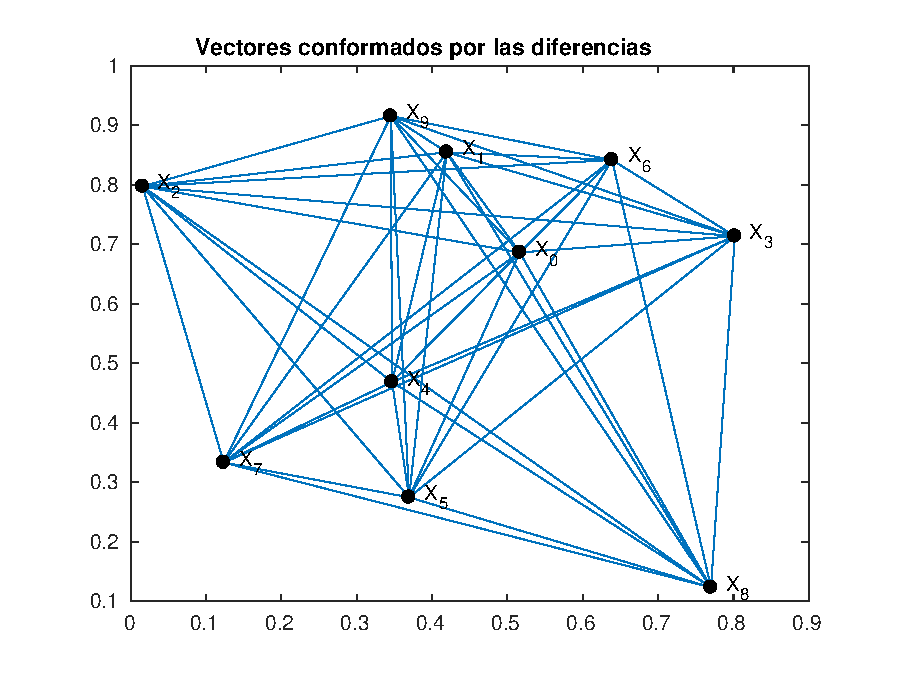
\includegraphics[width=0.5\textwidth]{Figures_Chapter6/Diferencias_Puntos.eps} &
   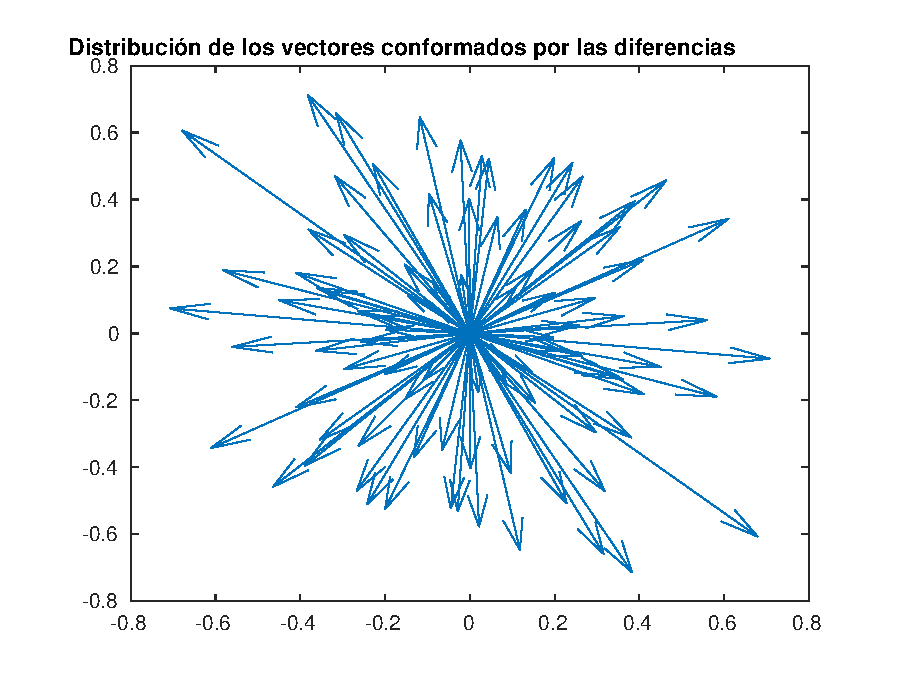
\includegraphics[width=0.5\textwidth]{Figures_Chapter6/Distribucion_Mutacion.eps} 
\end{tabular}
\caption{En la izquierda se muestra diez vectores, y en la parte derecha su correspondiente distribución de diferencias.}
\label{fig:Distribucion_Diferencias_Mutacion}
\end{figure*}

%
Las estrategias de mutaciones más utilizadas en la literatura son:
\begin{enumerate}
\item \textit{DE/rand/1}: $\boldsymbol{v}_{i,g} = \boldsymbol{x}_{r0,g} + F(\boldsymbol{x}_{r1,g} - \boldsymbol{x}_{2,g})$
\item \textit{DE/current-to-best/1}: $\boldsymbol{v}_{i,g} = \boldsymbol{x}_{r0,g} + F(\boldsymbol{x}_{best, g} - \boldsymbol{x}_{r2,g})  + F(\boldsymbol{x}_{r1,g} - \boldsymbol{x}_{r2,g})$
\item \textit{DE/best/1}: $\boldsymbol{v}_{i,g} = \boldsymbol{x}_{best, g} + F(\boldsymbol{x}_{r1,g} - \boldsymbol{x}_{r2,g})$
\end{enumerate}

%
Donde los índices $r_0$, $r_1$ y $r_2$ son enteros aleatorios y mutuamente exclusivos, escogidos del rango $[1, NP]$.
%
La diferencia de cualquiera par de estos tres vectores es escalado por un parámetro $F$ (normalmente es asignado en el intérvalo $[0.4, 1]$).
%

\subsubsection*{Operador de cruce en DE}

Para mejorar la diversidad de la población, se implementa el operador de cruce después de generar al vector donante.
%
El vector donante intercambia sus componentes con el vector objetivo $\boldsymbol{x}_{i,g}$ para formar al vector de prueba $\boldsymbol{u}_{i,g}$.
%
Así, la operacion de cruza binomial consiste en generar al vector de prueba final $\boldsymbol{u}_{i,g} = u_{1,i,g},  u_{2,i,g},... , u_{D,i,g}$, de la siguiente forma:
\[
   \boldsymbol{u}_{j, i, g} = 
\begin{cases}
      		\boldsymbol{v}_{j,i,g},& \text{si } \quad rand(0, 1) \leq CR_i \quad or \quad j=j_{rand}\\
    		\boldsymbol{x}_{j,i,g},& \text{de otra forma}
\end{cases}
\]
donde  $rand(0, 1)$ es generado de forma aleatoria con una distribución uniforme en el intervalo $[0, 1]$, $j_{rand} = randint(1, D)$ es un entero generado de forma aleatoria en el intervalo $[1, D]$ para cada vector $i$, y la probabilidad $CR_i \in [0,1]$ corresponde a la fracción de los componentes del vector que en promedio son heredados del vector mutado.
%
En DE clásico el parámetro $CR$ es un parámetro fijo para generar a todos los vectores de prueba, sin embargo existen variantes adaptativas donde cada individuo está asociado con su propia probabilidad de cruce $CR$.

%*Distribuiones empíricas con distintos valores de CR.
\subsubsection*{Selección en DE}
El operador de selección elige al mejor entre el vector padre $\boldsymbol{x}_{i,g}$ y el vector de prueba $\boldsymbol{u}_{i,g}$ de acuerdo a su aptitud.
%
En el caso de minimización un vector es seleccionado en base a lo siguiente:
\begin{equation}
   \boldsymbol{x}_{i, g+1} = 
\begin{cases}
      		\boldsymbol{u}_{i,g},& \text{si } f(\boldsymbol{u}_{i,g}) < f(\boldsymbol{x}_{i,g})\\
    		\boldsymbol{x}_{i,g},& \text{de otra forma}
\end{cases}
\end{equation}
el cual es utilizado en la siguiente generación como padre.
%%
%
\subsubsection*{Efecto de los parámetros}

Aunque DE es ampliamente utilizado en optimización de dominios continuos, para su implementación es necesario realizar un estudio de parametrización principalmente en problemas difíciles.
%
Una razón es que en problemas sencillos (ej. unimodal y de baja dimensionalidad) es necesario utiliza una población pequeña, pero en problemas complejos se recomiena aplicar una población grande para evitar que el proceso de búsqueda se estanque en un mínimo local.
%
Debido a que se incorpora el proceso de mutación con el de cruce, se puede interpretar al parámetro $CR$ como razón de mutación, siendo la probabilidad de heredar un parámetro del vector de donante.
%

En DE, el número promedio de parámetros mutados dado un valor de $CR$ depende en el esquema de cruce, sin embargo un valor pequeño de $CR$ corresponde a una razón de mutación pequeña.
%
\cite{storn1997differential} demostraron que todas las funciones pueden ser resueltas con $0 \leq CR \leq 0.2$ o $0.9 \leq CR \leq 1$.
%
Por otra parte una razón de mutación pequeña podría ser beneficioso para problemas que sean separables, es decir que no exista dependencia entre los parámetros ya que únicamente se cambiará un parámetro por cada vector.
%
A pesar de eso, pueden presentarse problemas de convergencia al implementar una razón de mutación pequeña, principalmente en los problemas con un grado elevado de dependencia.
%
\cite{salomon1996re} ha demostrado que una razón de mutación pequeña puede tener peores efectos que una búsqueda aletoria, principalmente en problemas de optimización no separables y multimodales.
%
Por lo tanto el valor $CR$ proporciona una forma de explotar la posibilidad de parámetros con independencia, y proporcionar una diversidad extra a la población en los vectores de prueba específicamente con $CR=1$ (\cite{price2006differential}), así en problemas con alta dependencia el valor $CR$ debe ser cercano a $1$.
%
Existen problemas que están orientados a sistemas de coordenadas especiales, por lo tanto el proceso de búsqueda deberá ser rotacionalmente invariante, es decir que el rendimiento no depende en la orientación de las coordenadas en donde se evalúa la función objetivo.
%
Esto se realiza con DE utilizando únicamente la mutación y no la cruza, esto significa que $CR=1$.
%
El efecto del parámetro $CR$ puede ser observado en la figura \ref{fig:Seleccion_Empirica}, donde se muestra la distribución empírica de los vectores de prueba o candidatos generados con el algoritmo estándar de evolución diferencial, considerando diez vectores en la población y $200$ generaciones, sin involucrar el proceso de selección.
%
Principalmente se observa que para valores de $CR=1$ el comportamiento del esquema DE/rand/1/bin es rotacionalmente invariante, mientras que para $CR=0.5$, el efecto es lineal, algo muy similar que en el operador SBX al heredar directamente información de los padres.

\begin{figure*}%[t]%[H]
\centering
\begin{tabular}{ccc}
   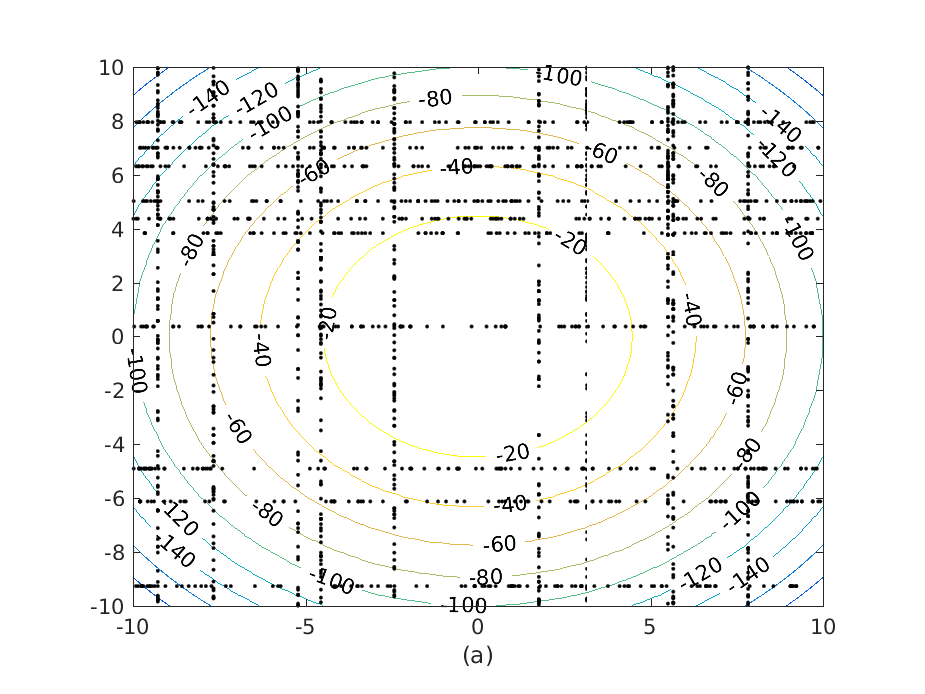
\includegraphics[width=0.33\textwidth]{Figures_Chapter6/Empirical_CR_0.eps} &
   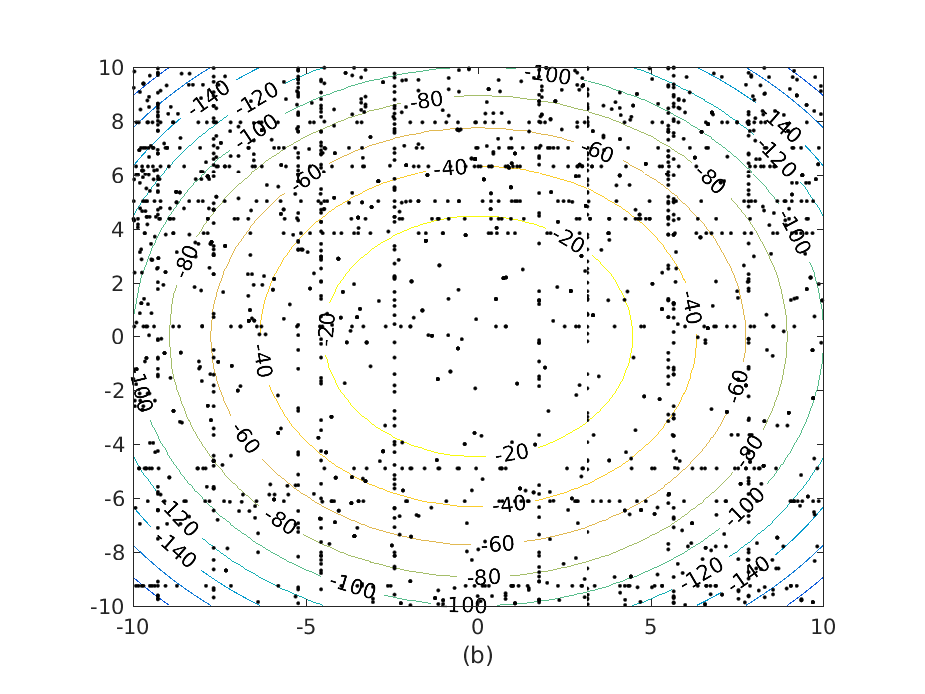
\includegraphics[width=0.33\textwidth]{Figures_Chapter6/Empirical_CR_05.eps} &
   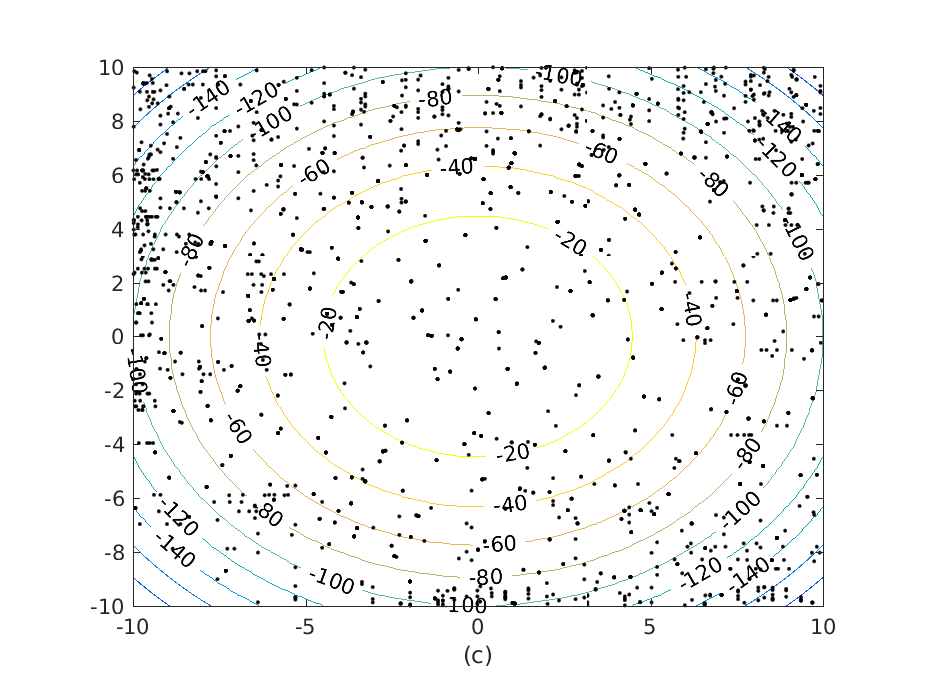
\includegraphics[width=0.33\textwidth]{Figures_Chapter6/Empirical_CR_1.eps} 
\end{tabular}
\caption{Distribución empírica de los vectores de prueba para los valores (a) CR = 0.0, (b) CR = 0.5, (c) CR = 1.0}
\label{fig:Seleccion_Empirica}
\end{figure*}

En base a la literatura el factor escala de mutación $F$ pertence al rango $(0,1)$, y aunque es posible asignar valores $F>1$ el rendimiento del algoritmo puede ser comprometido.
%
La cota inferior de este parámetro ha sido estudiado en detalle por \cite{zaharie2002critical}, ya que un valor pequeño tiende a reducir la diversidad de la población y para evitar la convergencia prematura, es importante que $F$ tenga una magnitud adecuada para contrarrestar la presión de selección.
%

Se ha establecido que si los valores $F$ y $NP$ son muy pequeños, la búsqueda se estancará en un mínimo local ya que con los parámetros de control pequeños el proceso de búsqueda converge sin alguna presión de selección (\cite{kukkonen2009performance}).
%
Así, \citeauthor{zaharie2002critical} estima el mínimo valor crítico mediante la fórmula $F_{crit} = \sqrt{ \frac{(1-\frac{CR}{2}}{NP}}$, aunque en la práctica es usualmente considerado como $F_{crit}=0.4$.
%

El factor escala de mutación puede ser transformado en una variable aleatoria de forma efectiva, este proceso puede favorecer en configuraciones con poblaciones pequeñas, de lo contrario DE podría estancarse.
%
Por lo tanto transformando $F$ en una variable aleatoria por medio una función de distribución, puede ayudar para demostrar una convergencia limitada (\cite{zaharie2002critical}).
%

El proceso de tranformar $F$ en una variable aleatoria es clasificado de dos formas.
%
En la primera se genera un valor $F$ para cada parámetro nombrado como \textit{jither}.
%
Alternativamente escoger un valor $F$ para cada vector  es conocido como \textit{dithering}.
%
Por lo tanto, la estrategia de dithering escala la longitud del vector de diferencias, por otra parte, jither escala a el vector de diferencias y cambia su orientación.
%
En base a varios análisis realizados por \cite{price2006differential}, se ha observado que implementar jither es efectivo en funciones separables, pero su rendimiento es pobre en funciones no separables y multimodales, en dado caso se recomienda implementar que la desviación de la distribución sea muy pequeña.
%
Por otra parte dithering es más estable y se ha observado que con una razón de mutación ($CR$) elevada puede superar a la forma usual que es fija.
%

\subsubsection*{Evolución diferencial en esquemas de diversidad explícita}

Aunque se han desarrollado técnicas para mantener un grado de diversidad en la población, no se ha analizado el comportamiento de los operadores de evolución diferencial con esquemas para mantener la diversidad de forma explícita.
%
Al mantener explícitamente la diversidad en la población pueden existir efectos no deseados al aplicar los operadores ya que inicialmente no se diseñaron para esquemas de largo plazo.
%
En un esquema usual de un EA, en las primeras generaciones los individuos de la población están bien distribuídos en el espacio factible, por lo tanto la distribución de los vectores de diferencia provocan desplazamientos elevados en el espacio de búsqueda, no obstante en función de la estrategia de selección estos desplazamientos tienden a ser menores, así conforme se detectan las regiones promisorias el comportamiento de los operadores de DE cambia de exploración a intensificación.
%
Esto sucede en base a las regiones óptimas encontradas en el proceso de búsqueda.

%
\begin{figure*}%[t]%[H]
\centering
\begin{tabular}{cc}
   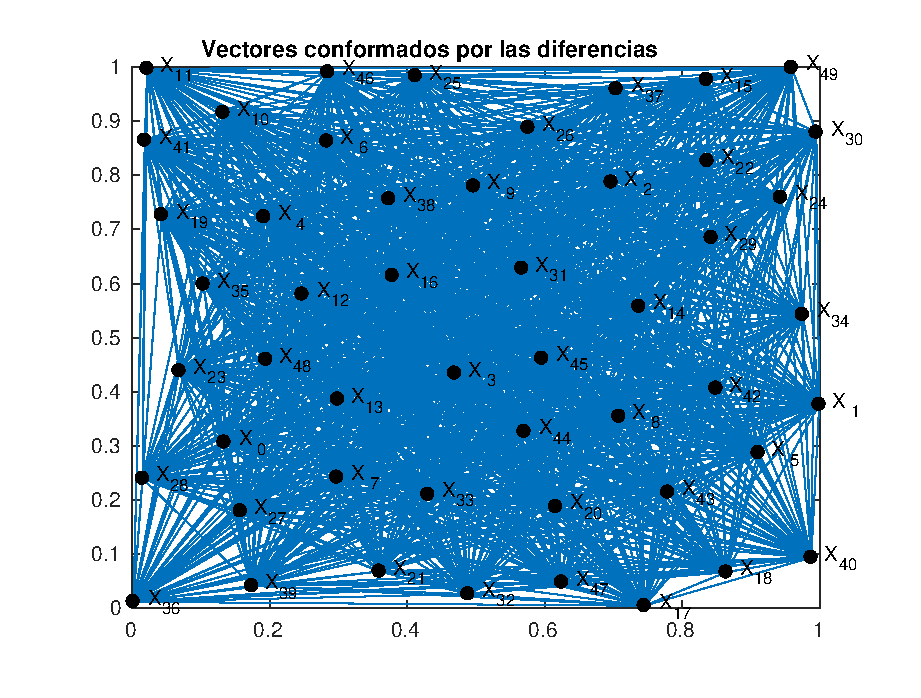
\includegraphics[width=0.5\textwidth]{Figures_Chapter6/Diferencias_Puntos_Diversidad.eps} &
   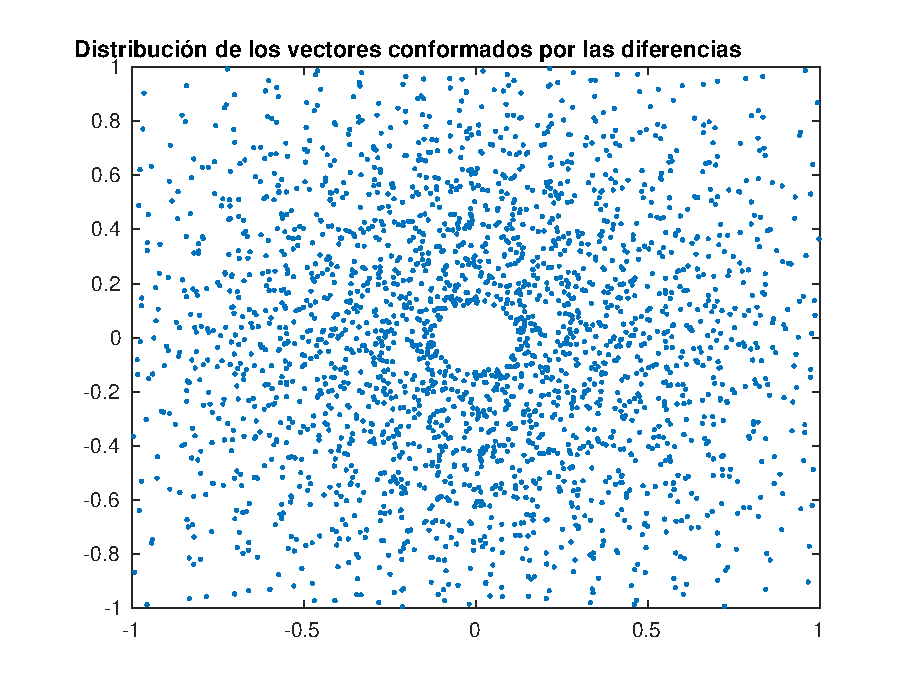
\includegraphics[width=0.5\textwidth]{Figures_Chapter6/Distribucion_Mutacion_Diversidad.eps} 
\end{tabular}
\caption{En la izquierda se muestran 50 vectores con una distancia mímina al vecino más cercano de $D_i = 0.125$, y en la parte derecha su correspondiente distribución de diferencias ($2450$), en la derecha cada punto corresponde a un vector de diferencia.}
\label{fig:Distribucion_Mutacion_Diversidad}
\end{figure*}


Por otra parte, en un esquema donde es mantenida la diversidad de forma explícita, se puede observar que en las primeras etapas de la ejecución los desplazamientos elevados pueden afectar la capacidad de búsqueda, ya que, dependiendo de la posición del vector base existirá una probabilidad elevada de ubicar a un individuo fuera del espacio factible.
%
Además, la distribución de los vectores de diferencias tendrán una longitud supeiror a la distancia mínima que existe entre cada individuo de la población, como se observa en la parte derecha de la figura \ref{fig:Distribucion_Mutacion_Diversidad}, aunque aplicar grandes desplazamientos puede ser favorable para fomentar la diversidad en la población, también es deseable generar vectores de diferencia pequeños, con el propósito de mejorar la aptitud de un individuo aislado y con una significativa contribución a la diversidad.
%
Esto implica que tanto los desplazamientos grandes como los pequeños son importantes en el proceso de búsqueda.
%
Para resolver las debilidades previamente mencionadas, se sugieren varias modificaciones al esquema clásico de DE.
%
Primeramente, se aplica un operador de mutación polinomial, así existirá un probabilidad de generar puntos en todo el espacio factible.
%

En base a que en las primeras fase del algoritmo se provocarán desplazamientos elevados y en consecuencia se generarán inidividuos fuera del espacio factible, se sugiere utilizar un mecanismo de reparo o posicionamiento adecuado como parte del proceso de exploración.

%
En la literatura (\cite{kreischerevaluation}) existen varias alternativas, una de los más utilizadas es el \textit{método de proyección}, el cual consiste en reasignar los componentes no factibles en el límite definida de la forma:
\begin{equation}
   \boldsymbol{v}_{i,j,g}= 
\begin{cases}
      		\boldsymbol{u}_{j},& \text{si } f(\boldsymbol{v}_{i,j,g}) >  \boldsymbol{u}_{j} \\
      		\boldsymbol{l}_{j},& \text{si } f(\boldsymbol{v}_{i,j,g}) <  \boldsymbol{l}_{j} \\
    		\boldsymbol{v}_{i,j,g},& \text{de otra forma}
\end{cases}
\end{equation}
donde $\boldsymbol{u}_j$ es el límite superior, $\boldsymbol{l}_j$ el límite inferior y $\boldsymbol{u}$ es el vector donante o mutado.
%
El método de proyección no es adecuado en este esquema de diversidad, ya que tiende a generar muchos individuos hijo en la frontera del espacio de búsqueda.
%
En su lugar se sugiere utilizar el método de \textit{base aleatorio}, este consiste en generar un valor aleatoriamente en el rango de los componentes aleatorios, este método es planteado de la siguiente forma:
\begin{equation}
   \boldsymbol{v}_{i,j,g} = 
\begin{cases}
      		\boldsymbol{base}_{j,g} + rand_{j}(0,1)( \boldsymbol{u}_j - \boldsymbol{base}_{j,g}),& \text{si } f(\boldsymbol{v}_{i,j,g}) >  \boldsymbol{u}_{j} \\
		\boldsymbol{base}_{j,g} + rand_{j}(0,1)( \boldsymbol{l}_j - \boldsymbol{base}_{j,g}), & \text{si } f(\boldsymbol{v}_{i,j,g}) <  \boldsymbol{l}_{j} \\
    		\boldsymbol{v}_{i,j,g},& \text{de otra forma}
\end{cases}
\end{equation}
%
Se puede observar que en esta propuesta no existe una tendencia al ubicar cualquier componente del vector mutado en el espacio factible, esto es deseable en esquemas a largo plazo, principalmente porque puede generar individuos diversos.
%

El comportamiento de la convergencia de un algoritmo de evolución diferencial está determinado principalmente por la configuración de los parámetros, como ya se ha analizado anteriormente algunas configuraciones son más adecuadas para para ciertos problemas.
%
Por otra parte, los algoritmos propuestos en este trabajo determinan el grado de convergencia manteniendo un grado de diversidad explícito, en base a esto se propone modificar el mecanismo usual de evolución diferencial.
%
Principalmente, la razón de mutación ($CR$), es asignada en base a dos estados como se indica en la ecuación (\ref{eq:estados}), donde el primer estado es principalmente para tratar problemas separables y el segundo será efectivo en problemas con una elevada dependencia entre las variables.
\begin{equation} \label{eq:estados}
   CR = 
\begin{cases}
      		0.2 ,& \text{si } rand(0,1) \leq 0.5 \\
    		1.0 ,& \text{de otra forma}
\end{cases}
\end{equation}
En la clásico DE, esta última modificación puede ocacionar problemas de convergencia, sin embargo en el esquema para mantener la diversidad de forma explítito favorece al proceso de exploración, además tiene la ventaja de requerir un parámetro menos como parte del algoritmo.
%

Por lo tanto, son sugeridos tres aspectos imporante para aplicar DE en esquemas con diversidad explícito:
\begin{itemize}
\item Utilizar el operador de mutación polinomial para tener una probabilidad de generar individuos en todo el espacio factible.
\item Aplicar un método de reparo que aporte al proceso de exploración.
\item La probabilidad que corresponde a la razón de mutación está conformada por dos estados.
\end{itemize}

%
%\section{Propuesta de evolución diferencial basado en esquemas de diversidad}

% Define some commands to keep the formatting separated from the content 
%\newcommand{\keyword}[1]{\textbf{#1}}
%\newcommand{\tabhead}[1]{\textbf{#1}}
%\newcommand{\code}[1]{\texttt{#1}}
%\newcommand{\file}[1]{\texttt{\bfseries#1}}
%\newcommand{\option}[1]{\texttt{\itshape#1}}

%----------------------------------------------------------------------------------------
